\documentclass{article}
\usepackage{graphicx}
\usepackage[a4paper, margin=2.5cm]{geometry}
\usepackage{fancyhdr}
\usepackage{lastpage}
\usepackage{hyperref}
\usepackage{polski}
\usepackage{amsmath}

\title{Metody numeryczne, projekt 2:\\Układy równań liniowych}
\author{Jakub Stachowicz\\198302}
\date{29 kwietnia 2025}

\pagestyle{fancy}
\fancyhf{} % Clear header and footer
\fancyfoot[C]{Strona \thepage\ z \pageref{LastPage}}

\renewcommand{\headrulewidth}{0pt} % Remove the horizontal bar at the top
\renewcommand{\footrulewidth}{0pt} % Remove the horizontal bar at the bottom if needed

\renewcommand{\contentsname}{Spis rzeczy} % Change the TOC title


\begin{document}
\maketitle
\newpage
\tableofcontents
\newpage
\section{Wstęp}
\subsection{Abstrakt}
Celem projektu jest implementacja i analiza trzech sposobów rozwiązywania układów równań liniowych, dwóch iteracyjnych (metoda Jacobiego i metoda Gaussa-Seidla) i jednej bezpośredniej (faktoryzacja LU).

\subsection{Analizowany układ równań}

W ogólności, układ równań liniowych ma następującą postać:
\begin{align}
       Ax = b,
\end{align}
gdzie $A$ jest macierzą systemową, $b$ jest wektorem pobudzenia, a $x$ jest wektorem rozwiązań.

Macierz $A$, która została przyjęta do użycia przy przeprowadzaniu analizy powyższych algorytmów, stanowi macierz pasmowa rozmiaru $N \times N$ o następującej strukturze\footnote{Wartość $N$ oraz elementów $a_1, a_2$ i $a_3$ zdefiniowane są w dalszej części opracowania.}:
\begin{align}
A=
\begin{bmatrix} 
a_1 & a_2 & a_3 & 0 & 0 & 0 & 0 & 0 & \dots & 0 \\ 
a_2 & a_1 & a_2 & a_3 & 0 & 0 & 0 & 0 & \dots & 0 \\ 
a_3 & a_2 & a_1 & a_2 & a_3 & 0 & 0 & 0 & \dots & 0 \\ 
0 & a_3 & a_2 & a_1 & a_2 & a_3 & 0 & 0 & \dots & 0 \\
0 & 0 & a_3 & a_2 & a_1 & a_2 & a_3 & 0 & \dots & 0 \\
\vdots & \vdots & \vdots & \vdots & \vdots & \vdots & \vdots & \vdots & \ddots & \vdots \\
0 & 0 & 0 & 0 & 0 & 0 & 0 & 0 & \dots & a_1
\end{bmatrix}
\end{align}

Jako wektor $b$, w tym samym celu, przyjęto wektor rozmiaru $N$ o wartościach będących kolejnymi elementami ciągu zadanego wzorem:
\begin{align}
    c_n = \sin(n\cdot(f+1)),
\end{align}
gdzie $f$ stanowi trzecią cyfrę indeksu autora sprawozdania ($f = 8$).

\subsection{Wektor residuum}
W metodach iteracyjnych korzysta się z wektora residuum, który obliczany jest w sposób następujący:
\begin{align}
    r = Ax - b.
\end{align}

Wyznaczona norma euklidesowa tego wektora pozwala stwierdzić, czy wyniki kolejnych iteracji zbiegają się do rozwiązania. Pozwala ona także przerwać działania iteracyjne, jeśli uzyskany zostanie wynik w wyznaczonej tolerancji. 

W dalszej części sprawozdania jako sygnał do zaprzestania obliczeń przyjęto normę residuum na poziomie mniejszym niż $10^{-9}$.

\section{Algorytmy}

\subsection{Metody iteracyjne}

Metody iteracyjne wykorzystują rozbicie macierzy $A$ na trzy podmacierze: macierz trójkątną dolną $L$, trójkątną górną $U$ i diagonalną $D$. Macierz $A$ stanowi ich sumę.
\begin{align}
    A = L + U + D
\end{align}

\subsubsection{Metoda Jacobiego}
Po przekształceniach wzoru (5) i podstawieniu go do wzoru (1):
\begin{align}
    Dx &= -(L + U)x + b \\
    x &= -D^{-1}(L + U)x + D^{-1}b,
\end{align}
otrzymujemy następujący wzór na oszacowanie wektora rozwiązań $x$ w $(k+1)$-szej iteracji, na bazie wektora z $k$-tej iteracji.
\begin{align}
    x^{(k+1)} = -D^{-1}(L + U)x^{(k)} + D^{-1}b = M_Jx^{(k)} + w_J.
\end{align}

Jako wektor początkowy przyjmuje się wektor długości $N$ o zawartości jedynek.

\subsubsection{Metoda Gaussa-Seidla}
Po przekształceniach wzoru (5) i podstawieniu go do wzoru (1):
\begin{align}
    (D+L)x=-Ux+b
\end{align}
otrzymujemy następujący wzór na oszacowanie wektora rozwiązań $x$ w $(k+1)$-szej iteracji, na bazie wektora z $k$-tej iteracji.
\begin{align}
    x^{(k+1)} = -(D+L)^{-1}(Ux^{(k)}) + -(D+L)^{-1}b = M_{GS}x^{(k)} + w_{GS}.
\end{align}

Jako wektor początkowy, podobnie jak w metodzie Jacobiego, przyjmuje się wektor długości $N$ o zawartości jedynek.

\subsection{Metoda bezpośrednia (faktoryzacja LU)}
Metoda ta polega na utworzeniu takich macierzy trójkątnych $L$ i $U$, żeby zachodziło równanie $LUx = b$. 

Tworzy się wówczas wektor pomocniczy $y = Ux$, a następnie rozwiązuje układ równań $Ly = b$ za pomocą podstawiania wprzód, a następnie -- układ $Ux = y$ za pomocą podstawiania wstecz.

Sednem tego algorytmu jest faktoryzacja macierzy $A$ na macierze $L$ i $U$. Można tego dokonać stosując poniższy algorytm (w Pythonie):
\begin{verbatim}
def LU_decomposition(A, m):
    U = copy.copy(A)
    L = np.eye(m)
    for i in range(2, m + 1):
        for j in range(1, i):
            L[i - 1, j - 1] = U[i - 1, j - 1] / U[j - 1, j - 1]
            U[i - 1, :] = U[i - 1, :] - L[i - 1, j - 1] * U[j - 1, :]
    return L, U
\end{verbatim}
Taki też został zastosowany w dalszej analizie tego algorytmu.

\section{Analiza}
\subsection{Metody iteracyjne}

\textbf{Pierwsza analiza}

Jako rozmiar macierzy $N$ przyjęto liczbę $1200 + 10c + d$, gdzie $c$ jest przedostatnią cyfrą numeru indeksu autora, a $d$ -- ostatnią. Ostatecznie $N = 1202$. Jako $a_2$ i $a_3$ przyjęto $-1$, a jako $a_1$ -- liczbę o 5 większą od czwartej cyfry numeru indeksu autora. Ostatecznie $a_1 = 8$.

Zarówno metoda Jacobiego, jak i metoda Gaussa-Seidla poradziły sobie z rozwiązaniem zadanego układu równań. 

Metoda Jacobiego okazała się szybsza czasowo (rozwiązanie podała w 202 ms w przeciwieństwie do 1431 ms), jednak dotarcie do zadowalającej odpowiedzi (tj. takiej, w której norma residuum wynosi mniej niż $10^{-9}$) zajęło jej więcej iteracji (38, w przeciwieństwie do 24).

Obie te metody zbiegały się w podobny sposób -- wykładniczo -- co przedstawiają wykresy 1 i 2 (w skali logarytmicznej).

Metody iteracyjne nie są jednak uniwersalnym sposobem rozwiązywania układów równań liniowych, o czym świadczy druga analiza.

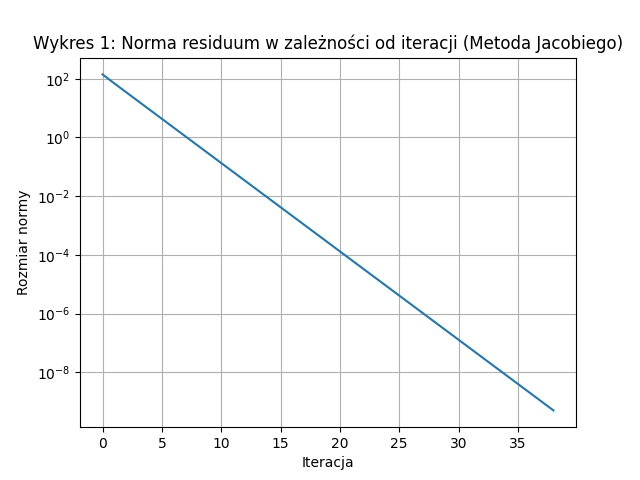
\includegraphics[scale=0.67]{chart1.png}

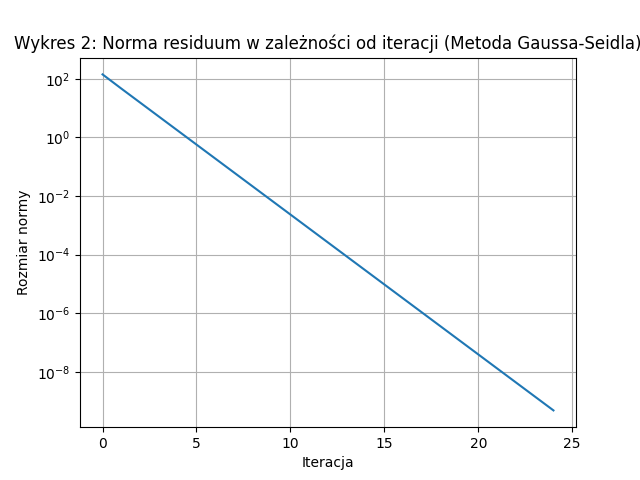
\includegraphics[scale=0.67]{chart2.png}

\textbf{Druga analiza}

Niech $N$ pozostanie takie jak w pierwszej analizie, podobnie $a_2$ i $a_3$, ale niech $a_1$ wynosi 3.

Dla obu podanych metod, wraz ze wzrostem liczby iteracji, wykładniczo rośnie wartość normy residuum, co świadczy o rozbieżności. Ogromny rozmiar tejże rozbieżności zaobserwować można na wykresach 3 i 4 (w skali logarytmicznej).

Wykonywanie algorytmów zostaje przerwane po 200 iteracjach, jako przyjęty limit długości obliczeń w przypadku nieosiągnięcia warunku zadowalającej normy residuum.

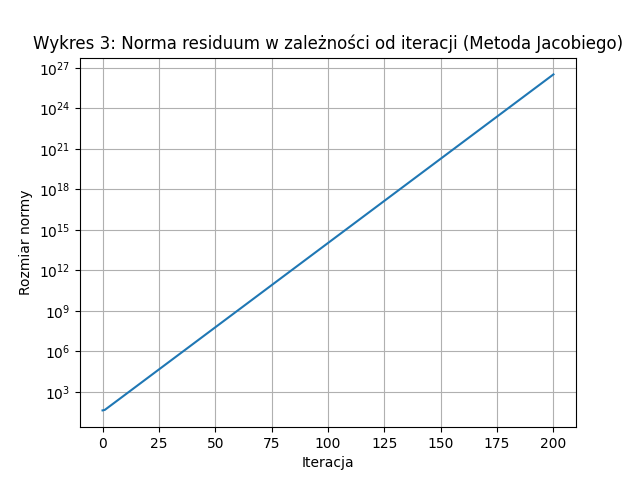
\includegraphics[scale=0.67]{chart3.png}

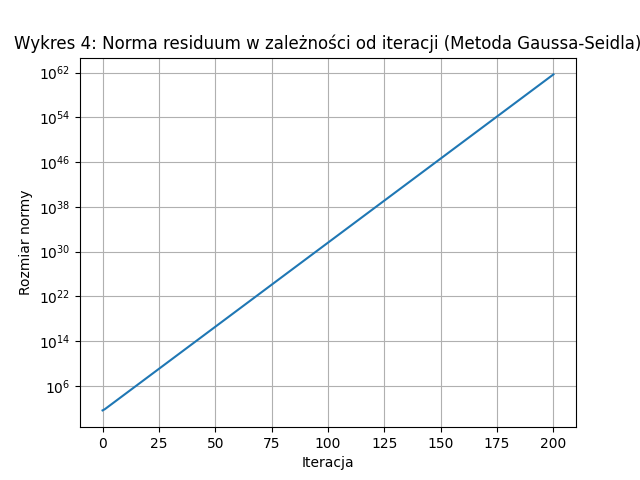
\includegraphics[scale=0.67]{chart4.png}

\subsection{Metoda bezpośrednia (faktoryzacja LU)}

Do rozwiązania układu równań zastosowanego w drugiej analizie metod iteracyjnych zastosowana zostałą również metoda bezpośrednia (faktoryzacja LU). 

Obliczenia trwały 4468 ms, jednak metoda ta zwróciła poprawny wynik. Norma residuum wyniosła $1,174 \cdot 10^{-12}$.

Oznacza to, że ta metoda, choć będąca zwykle wolniejsza od metod iteracyjnych, ma większe szanse powodzenia znalezienia poprawnego rozwiązania, gdyż nie bazuje na pewnej heurystyce związanej ze stabilnością obliczeniową.

\subsection{Analiza wydajności}

Podczas analizy wydajności wszystkich trzech metod skonstruowano ciąg macierzy o rozmiarach $N = 100, 500, 1000, 2000, 3000$. Parametry $a_n$ zdefiniowano w ten sam sposób, co w pierwszej analizie metod iteracyjnych (sekcja 3.1).

Wszystkie te układy równań zostały poprawnie rozwiązane przez wszystkie trzy analizowane algorytmy.

Dla każdego rozmiaru macierzy badany algorytm uruchamiany był 10 razy, następnie obliczona średnia czasu wykonania została umieszczona na wykresach (5 -- w skali logarytmicznej, 6 -- w skali naturalnej).

Zaobserwować można silny wzrost czasu wykonania metody bezpośredniej. Metody iteracyjne są szybsze, zwłaszcza (na sprzęcie i oprogramowaniu autora sprawozdania) metoda Jacobiego.

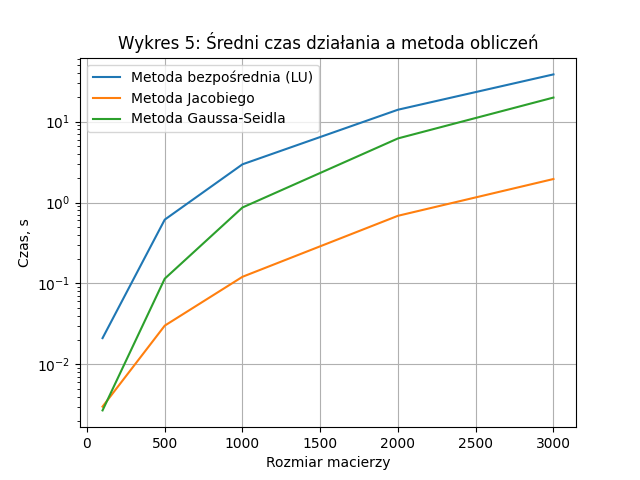
\includegraphics[scale=0.67]{chart5.png}

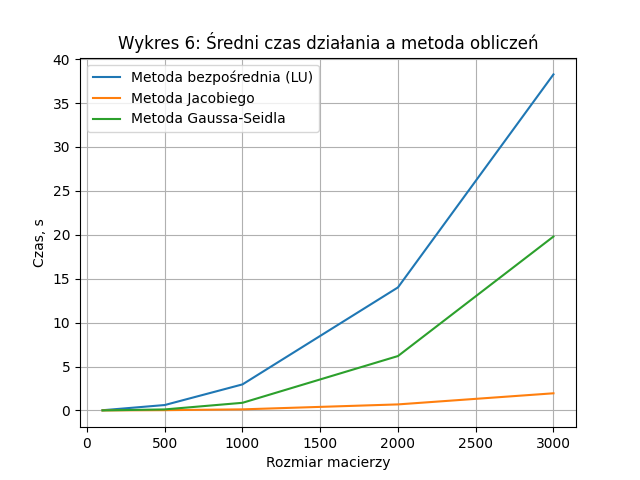
\includegraphics[scale=0.67]{chart6.png}

\section{Podsumowanie}

Na podstawie przeprowadzonych analiz można stwierdzić, że metody iteracyjne (Jacobiego i Gaussa-Seidla) są znacznie szybsze w znajdowaniu rozwiązań układów równań niż metoda bezpośrednia (faktoryzacja LU). Czas działania wynika z ich złożoności obliczeń, która dla metody bezpośredniej wynosi O($n^3$), a w przypadku metod iteracyjnych -- O($n^2$).

Metody iteracyjne jednak nie zawsze znajdują poprawne rozwiązanie wyniku, są przez to mniej uniwersalne. Warto jednak z nich skorzystać i poznać zwrócony przez nie wynik, wraz z normą. Nakład pracy jest znacznie mniejszy niż w przypadku metody bezpośredniej, więc warto jest zaryzykować, a następnie skorzystać z metody bezpośredniej tylko wówczas, jeśli z normy residuum wynika, iż rozwiązanie się nie zbiegło.



\section{Bibliografia}
\begin{enumerate}
\item Fotyga G., 2024: Wykład ,,\textit{Układy Równań Liniowych, Metody Numeryczne}''.
\item Fotyga G., 2025: Instrukcja ,,\textit{Metody Numeryczne, Projekt 2 -- Układy równań liniowych}''.
\item Fotyga G., Sypek P., 2025: Instrukcja ,,\textit{Metody numeryczne, laboratorium 3.
Metody rozwiązywania równania macierzowego}''.

\end{enumerate}
\end{document}
